\documentclass[a4paper,12pt]{article} % тип документа

% Поля страниц
\usepackage[left=2.5cm,right=2.5cm,
    top=2cm,bottom=2cm,bindingoffset=0cm]{geometry}
 
    
%Отступ после заголовка    
\usepackage{indentfirst}


% Рисунки
\usepackage{floatrow,graphicx,calc}
\usepackage{wrapfig}

% Создаёем новый разделитель
\DeclareFloatSeparators{mysep}{\hspace{1cm}}

% Ссылки?
\usepackage{hyperref}
\usepackage[rgb]{xcolor}
\hypersetup{				% Гиперссылки
    colorlinks=true,       	% false: ссылки в рамках
	urlcolor=blue          % на URL
}


%  Русский язык
\usepackage[T2A]{fontenc}			% кодировка
\usepackage[utf8]{inputenc}			% кодировка исходного текста
\usepackage[english,russian]{babel}	% локализация и переносы


% Математика
\usepackage{amsmath,amsfonts,amssymb,amsthm,mathtools}


% Что-то 
\usepackage{wasysym}


%Заговолок
\author{Серебренников Даниил Б02-826}
\title{Лабораторная работа \No 2.2.3}


\begin{document}


\begin{center}
\footnotesize{ФЕДЕРАЛЬНОЕ ГОСУДАРСТВЕННОЕ АВТОНОМНОЕ ОБРАЗОВАТЕЛЬНОЕ 			УЧРЕЖДЕНИЕ ВЫСШЕГО ОБРАЗОВАНИЯ}\\
\footnotesize{МОСКОВСКИЙ ФИЗИКО-ТЕХНИЧЕСКИЙ ИНСТИТУТ\\(НАЦИОНАЛЬНЫЙ 			ИССЛЕДОВАТЕЛЬСКИЙ УНИВЕРСИТЕТ)}\\
\footnotesize{ФАКУЛЬТЕТ ОБЩЕЙ И ПРИКЛАДНОЙ ФИЗИКИ\\}
\hfill \break
\hfill\break
\hfill\break
\hfill \break
\hfill \break
\hfill \break
\hfill \break
\hfill \break
\hfill \break
\hfill \break
\hfill \break
\hfill \break
\hfill \break
\hfill \break
\hfill \break
\large{Лабораторная работа № 2.2.1\\\textbf{Исследование взаимной диффузии газов}}\\
\hfill \break
\hfill \break
\hfill \break
\begin{flushright}
	Серебренников Даниил\\
	Группа Б02-826
\end{flushright}
\hfill \break
\hfill \break
\hfill \break
\hfill \break
\hfill \break
\end{center}
\hfill \break
\hfill \break
\hfill \break
\hfill \break
\hfill \break
\begin{center}
	Долгопрудный, 2019 г.
\end{center}
\thispagestyle{empty} % выключаем отображение номера для этой страницы


\newpage
\textbf{Цель работы:} 1) регистрация зависимости концентрации гелия в воздухе от времени с помощью датчиков теплопроводности при разных начальных давлениях смеси газов; 2) определение коэффициента диффузии по результатам измерений.

\textbf{В работе используются:} измерительная установка; форвакуумный насос; балон с газом 	(гелий); манометр; источник питания; магазин сопротивлений; гальванометр; секундомер.


\section{Теоретическая часть}
	\textit{Диффузией}  называют самопроизвольное взаимное проникновение веществ друг в друга происходящее вследствие хаотичного теплового движения молекул. При перемешивании молекул разного сорта говорят о взаимной (или концентрационной) диффузии. В системе, состоящей из двух компонентов a и b (бинарная смесь), плотности потоков частиц в результате взаимной диффузии определяются законом Фика:
	\begin{equation}
		j_a = -D \frac{\partial n_a}{\partial x}, \, j_b = -D \frac{\partial n_b}{\partial x},
	\end{equation}
	где $D$ — \textit{коэффициент взаимной диффузии компонентов}. Знак <<минус>> отражает тот факт, что диффузия идёт в направлении выравнивания концентраций. Равновесие достигается при равномерном распределении вещества по объёму.
	
	В данной работе исследуется взаимная диффузия гелия и воздуха. Отметим, что давление и температура в системе предполагаются неизменным: $P_0 = (n_{He}+n_{Air})kT = const$, где $n_{He}$  и $n_{Air}$ -- концентрации диффундирующих газов. Поэтому для любых изменений концентраций справедливо $\Delta n_{Air} = -\Delta n_{He}$. Следовательно, достаточно ограничиться описанием диффузии одного из компонентов, например гелия.
	
	Приведём теоретическую оценку для коэффициента диффузии. В работе концентрация гелия, как правило, мала ($n_{He} \ll n_{Air}$). Кроме того, атомы гелия легче молекул, составляющих воздух ($m_{He} \ll m_{N_2}, m_{O_2}$), значит их средняя тепловая скорость велика по сравнению с остальными частицами. Поэтому перемешивание газов в работе можно приближенно описывать как диффузию примеси лёгких частиц He на практически стационарном фоне воздуха. Коэффициент диффузии в таком приближении равен
	\begin{equation}
		\label{D}
		D = \frac{1}{3} \lambda \langle v \rangle,
	\end{equation}
	где $\lambda = \frac{1}{n\sigma}$ -- длина свободного пробега диффундирующих частиц; $\langle v \rangle = \sqrt{\frac{8kT}{\pi m}}$ -- их средняя тепловая скорость.
	
	Предпологая, что процесс диффузии будет квазиостационарным, можно показать, что разность концентраций будет убывать по экспоненциальному закону
	\begin{equation}
		\label{Delta_n}
		\Delta n = \Delta n_0 e^{-t / \tau},
	\end{equation}
	где $\tau$ -- характерное время выравнивания концентраций между сосудами, определяемое следующей формулой
	\begin{equation}
		\label{Tau}
		\tau = \frac{1}{D} \frac{VL}{2S}.
	\end{equation}
	
\section{Модель эксперимента}
	Для   исследования   взаимной диффузии газов и измерения коэффициента взаимной диффузии  $D$  используется  два сосуда  объёмами  $V_1$ и $V_2$ ($V_1 \approx V_2 := V$), соединенные трубкой длины $L$ и сечения  $S$. Предполагается, что сосуды заполнены смесью двух газов при одинаковом давлении, но с различной концентрацией компонентов. Вследствие взаимной диффузии, проходящей в   соединительной трубке, концентрации компонентов в сосудах с течением времени выравниваются.

	Для измерения разности  концентраций  в установке применяются датчики теплопроводности. При этом используется тот факт, что теплопроводность смеси $\kappa$ зависит от её состава. В общем случае   зависимость  $\kappa (n)$  довольно   сложна,   однако   при   малой   разности  $\Delta n$ концентраций в сосудах можно ожидать, что разность теплопроводностей будет изменяться прямо пропорционально $\Delta n:$
	\begin{equation*}
		\Delta \kappa = \kappa (n_2) - \kappa (n_1) \approx const \cdot \Delta n.
	\end{equation*}	 
	
	Эксперименты показывают, что если доля примеси гелия составляет менее 15\%, отклонение от линейной зависимости не превышает 0,5\%, что для наших целей вполне достаточно.
	
%Сами датчики теплопроводности устроены следующим образом. Тонкая платиновая  проволочка, протянутая вдоль оси стеклянного цилиндра, нагревается током. Внутренняя полость датчика сообщается с объёмом камеры через отверстия, размеры которых таковы, что скорость диффузии  из объёма сосуда в полость датчика значительно больше скорости диффузии из одного объёма в другой. Таким образом, состав газа в датчике практически совпадает с составом газа в объёме. Тепло от проволочки к стенке цилиндра передаётся главным образом за счёт теплопроводности газа, находя-щегося внутри цилиндра.% 

	При заданной мощности нагревания приращение температуры  проволочки и, следовательно, приращение её сопротивления пропорциональны теплопроводности газа. Для измерения сопротивлений используется мостовая схема, позволяющая определять разность показаний датчиков с высокой точностью. Мост балансируется при заполнении сосудов (и датчиков) одной и той же смесью. При заполнении сосудов смесями различного состава возникает «разбаланc» моста. При незначительном различии в составах смесей показания гальванометра, подсоединённого к диагонали моста, будут пропорциональны разности концентраций примеси: $U\propto\Delta \kappa \propto \Delta n$. В процессе диффузии разность концентраций убывает по закону~(\ref{Delta_n}), и значит по тому же закону изменяются во времени показания гальванометра
	\begin{equation}
		U = U_0 \, e^{-t / \tau},
	\end{equation}		
	где $U_0$ -- показание в начальный момент времени. Измеряя экспериментально зависимость $U(t)$, можно получить характерное время процесса $\tau$, откуда по формуле~(\ref{Tau}) определить коэффициент диффузии $D$.

\newpage
\section{Экспериментальные данные}
	В таблице~\ref{table:parametri} приведены некоторые параметры установки и случайные ошибки измерения величин, определяемых в ходе эксперимента.
	\floatsetup[table]{capposition=top}	
	\begin{table}[H]
		\caption{Некоторые параметры установки и ошибки измерений.}
		\label{table:parametri}
		\begin{tabular}{|c|c|c|c|c|}
			\hline
                  			  & $T$, К & $P_0$, торр & $V$, см$^3$ & $L/S$, 1/см \\ \hline
			Величина          & 293    & 760         & 775         & 5,3         \\ \hline
			Погрешность       & 0      & 0           & 10          & 0,1         \\ \hline
			$\varepsilon$, \% & 0      & 0           & 1,3         & 1,9         \\ \hline
		\end{tabular}
	\end{table}	
	На рисунке~\ref{ris:Graph_1} представлены графики зависимости $\ln U$ от $t$, построенные при различных рабочих давлениях $P$. Аппроксимированная прямая была построена методом наименьших квадратов. Экспериментальные данные были получены в компьютерной программе, предназначенной для данной лабораторной работы.
	\begin{figure}[H]
		\center{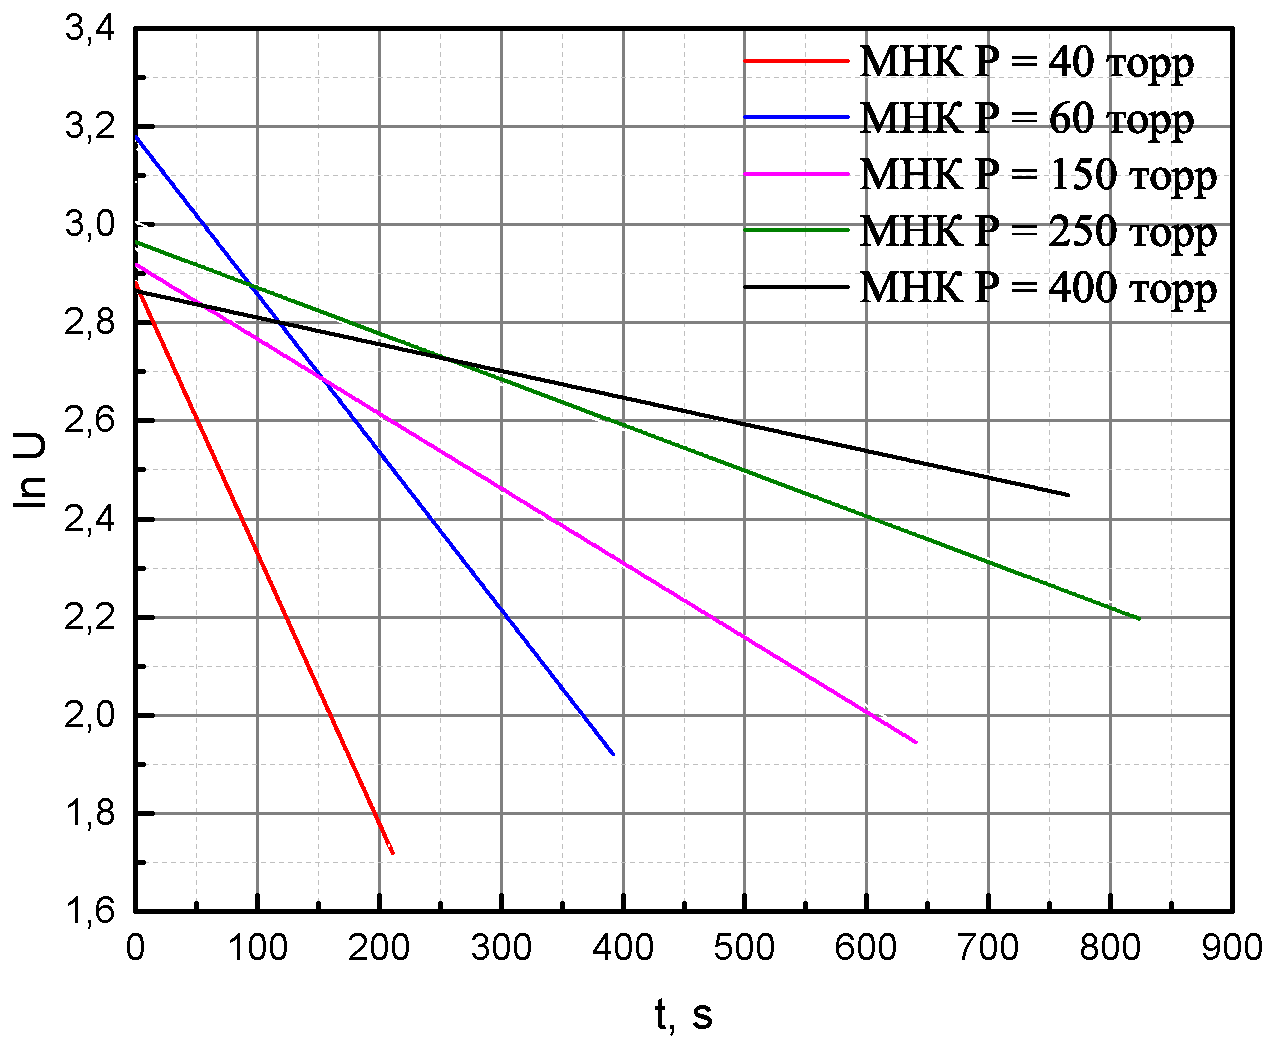
\includegraphics[scale=0.5]{Graph_1.pdf}}
		\caption{Зависимости $\ln U$ от $t$.}
		\label{ris:Graph_1}
	\end{figure}
	Результаты анализа графиков и результаты вычислений коэффициентов диффузии представлены в таблице~\ref{table:analis_of_graph}. Погрешностью наклонов графиков можно пренебречь в силу их малой относительной погрешности $\varepsilon = 0,1 \% $.
	\floatsetup[table]{capposition=top}	
	\begin{table}[H]
		\caption{Результаты анализа прямых (рис.~\ref{ris:Graph_1}).}
		\label{table:analis_of_graph}
		\begin{tabular}{|c|c|c|c|c|c|}
			\hline
				$P$, торр & $d\ln U /dt$ & $\tau$, с & $1/P$, торр$^{-1}$ & $D$, см$^2$/с & $\varepsilon_D$, \% \\ \hline
				40        & -0,005508    & 181,55    & 0,0250             & 11,3          & 2,3                 \\ \hline
				60        & -0,003214    & 311,16    & 0,0167             & 6,60          & 2,3                 \\ \hline
				150       & -0,001522    & 657,17    & 0,0067             & 3,13          & 2,3                 \\ \hline
				250       & -0,000932    & 1072,49   & 0,0040             & 1,91          & 2,3                 \\ \hline
				400       & -0,000544    & 1838,95   & 0,0025             & 1,12          & 2,3                 \\ \hline
		\end{tabular}
	\end{table}
	По полученным значениям коэффициентов диффузии построим график (рис.~\ref{ris:Graph_2}) зависимости $D$ от $1/P$.
	\begin{figure}[H]
		\center{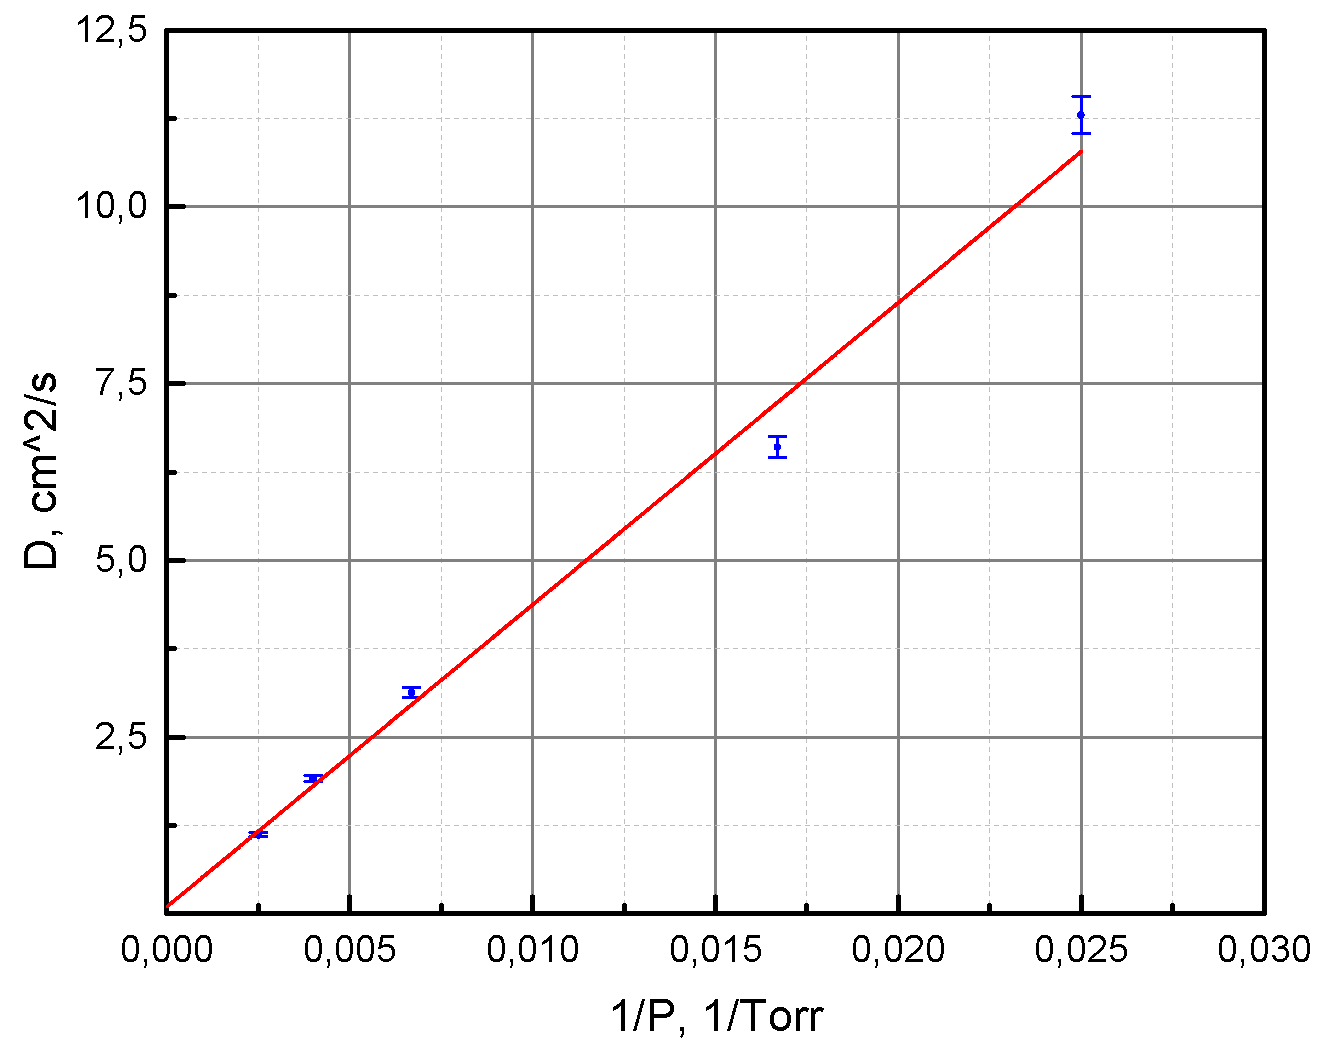
\includegraphics[scale=0.5]{Graph_2.pdf}}
		\caption{Зависимости $D$ от $1/P$.}
		\label{ris:Graph_2}
	\end{figure}
	 По графику методом наименьших квадратов определим коэффциент взаимной диффузии гелия с воздухом при атмосферном давлении $P_0$. Погрешность оценим по следующей формуле $\sigma_D = \frac{1}{P_0} \sigma_a + \sigma_b$, где $a$ и $b$ - коэффициенты, задающие прямую $D = a\frac{1}{P} + b$.
	\floatsetup[table]{capposition=top}	
	\begin{table}[H]
		\caption{Результаты анализа прямой (рис.~\ref{ris:Graph_2}).}
		\label{table:results}
		\begin{tabular}{|c|c|c|c|c|c|c|}
			\hline
			$a$, см$^2 \cdot$торр/c & $\sigma_a$, см$^2 \cdot$торр/c & $b$, см$^2$/c & $\sigma_b				$, см$^2$/c & $D$, см$^2$/c & $\sigma_D$, см$^2$/c & $\varepsilon$, \% \\ \hline
			427                     & 26                             & 0,10          & 0,12                 & 0,66          & 0,15                 & 23                \\ \hline
		\end{tabular}
	\end{table}
	Дополнительно можно вычислить длину свободного пробега гелия при комнатной температуре и атмосферном давлении в воздухе $\lambda$ и эффективное сечение столкновений атомов гелия с частицами воздуха $\sigma$. Результаты вычислений представлены в таблице~\ref{table:dopolnitelno}.
	\floatsetup[table]{capposition=top}	
	\begin{table}[H]
		\caption{Дополнительные характерные параметры гелия в воздухе.}
		\label{table:dopolnitelno}
		\begin{tabular}{|c|c|c|c|c|}
			\hline
			$\langle v \rangle$, м/c & $\lambda$, нм & $\sigma_\lambda$, нм & $\sigma$, $10^{-15}$ см$^2$ & $\sigma_\sigma$, $10^{-15}$ см$^2$ \\ \hline
			1328,5                  & 150           & 30                    & 2,7                         & 0,5                                \\ \hline
		\end{tabular}
	\end{table}
	
\section*{Обсуждение результатов}
	В ходе лабораторной работы нам удалось определить коэффициент взаимной диффузии $D$ гелия и воздуха при комнатной температуре и давлении, равном физической атмосфере. Полученный результат $D = (0,66 \pm 0,15)$ см$^2$/c в пределах погрешности сходится с табличным значением $D = 0,62$ см$^2$/c. Не мало важным фактом является то, что наша прямая (рис.~\ref{ris:Graph_2}) смещена на некоторую константу относительно нуля, поэтому наибольшую погрешность вносит этот сдвиг. Если проэкстраполировать прямую, считая, что она обязана пройти через нуль из теоретических соображений, то $D = (0,58 \pm 0,01)$ см$^2$/c.
	
	Однако всё же среднее значение полученной нами величины превышает табличное на 6,5 \%. Очевидно, что это в первую очередь связано с течами газа через краны, которые не идеально изолируют балоны. Кроме того, у установки отсутствуют пассивная и активная виброзащиты, поэтому любые колебания стола, на котором находится установка, приводят к искажению показаний вольтметра. Стоит отметить, что в силу неполного обмена энергией между молекулами газа и поверхностью нити её температура несколько выше, чем температура прилегающих слоёв газа -- на её поверхности возникает температурный скачок, который может исказить так же результаты.
	
	Мы дополнительно оценили длину свободного пробега гелия при комнатной температуре и атмосферном давлении в воздухе $\lambda = (150 \,\pm \, 30)$нм и эффективное сечение столкновений атомов гелия с частицами воздуха $\sigma = (2,7 \, \pm \, 0,5) \cdot 10^{-15}$см$^2$. 
	
\section*{Выводы}
	\enumerate
		\item
			Определили коэффициент взамной диффузии гелия и воздуха, который с учётом погрешности сходится с табличным значением: $D = (0,58 \pm 0,01)$ см$^2$/с.
		\item
			Рассчитали длину свободного пробега гелия при комнатной температуре и атмосферном давлении в воздухе $\lambda = (150 \,\pm \, 30)$нм.
		\item
			Рассчитали эффективное сечение столкновений атомов гелия с частицами воздуха $\sigma = (2,7 \, \pm \, 0,5) \cdot 10^{-15}$см$^2$.

































\end{document}
